\begin{question}
\noindent A circular observatory dome is being designed for a space exploration museum, alongside a display area shaped as a sector, used to showcase a history-of-astronomy exhibition of novels and star charts.

The circular base of the dome has circumference $C = (2x + 44)$ cm, where $x$ is a positive integer.

\begin{center}
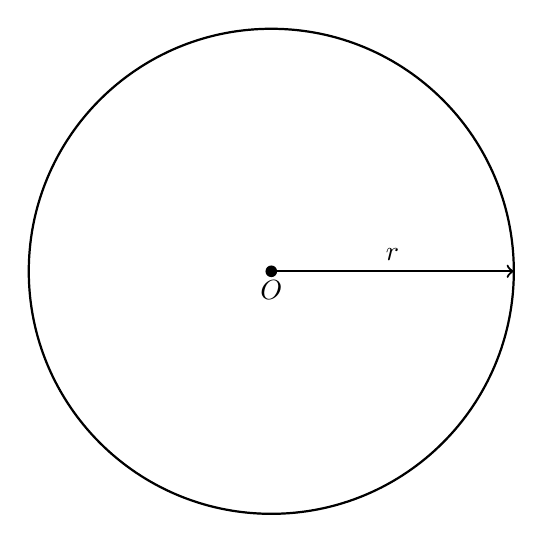
\begin{tikzpicture}[scale=1.4]
    \coordinate (O) at (0,0);
    \draw[thick] (O) circle (2.2);
    \fill (O) circle (1.5pt);
    \node at (O) [below] {$O$};
    \draw[thick, ->] (O) -- (2.2,0) node[midway, above] {$r$};
    \node at (1.6, 1.6) {};
    \draw[dashed] (0,0) circle (2.2);
\end{tikzpicture}
\end{center}

\noindent The radius of the dome, in cm, is given by $r = \dfrac{x}{5} + 3$.

\begin{enumerate}
    \item[(a)] Using the formula for circumference, $C = 2\pi r$, form an equation in $x$ and show that it simplifies to
    \[
    2x + 44 = 2\pi\left(\frac{x}{5} + 3\right)
    \]
    Hence find the value of $r$, giving your answer to 3 significant figures.
    \vspace{4cm}
    \answerequnit{r}{cm}{3}

    \item[(b)] Using your value of $r$ from part (a), calculate the area of the circular base of the dome.

    Give your answer to 3 significant figures.
    \vspace{3.5cm}
    \answerequnit{A}{cm^2}{1}

    \item[(c)] The museum planner claims that the area of the dome's base, in cm$^2$, is always greater than $30r^2$ for any positive value of $r$.

    Show that this claim is correct.
    \vspace{3cm}
    \answermarks{1}
\end{enumerate}
\end{question}
